%   This file is part of the APS files in the REVTeX 4.1 distribution.
%   Version 4.1r of REVTeX, August 2010
%
%   Copyright (c) 2009, 2010 The American Physical Society.
%
%   See the REVTeX 4 README file for restrictions and more information.
%
\documentclass[%
preprint,
onecolumn,
%superscriptaddress,
%groupedaddress,
%unsortedaddress,
%runinaddress,
%frontmatterverbose, 
% preprint,
%showpacs,preprintnumbers,
%nofootinbib,
%bibnotes,
%nobibnotes,
amsmath,amssymb,
aps,
%pra,
%prb,
%rmp,
%prstab,
%prstper,
%floatfix
]{revtex4-1}

%%%%%%%%%%%%%%%%%%%%%%%%%%%%%%%%%%%%%%%%%%%%%
% IMPORTS
\usepackage{graphicx}          % Include figure files
\usepackage{dcolumn}           % Align table columns on decimal point
\usepackage{bm}                % bold math
\usepackage{siunitx}           % SI unit handling
% \usepackage{hyperref}          % add hypertext capabilities
% \usepackage[mathlines]{lineno} % Enable numbering of text and display math
% \linenumbers\relax             % Commence numbering lines

\usepackage{lmodern}           % Font package
\usepackage{floatrow}
\usepackage{capt-of}
% Non-standard geometry import
% \usepackage[showframe,%Uncomment any one of the following lines to test 
% scale=0.7, marginratio={1:1, 2:3}, ignoreall,% default settings
% %text={7in,10in},centering,
% %margin=1.5in,
% %total={6.5in,8.75in}, top=1.2in, left=0.9in, includefoot,
% %height=10in,a5paper,hmargin={3cm,0.8in},
% ]{geometry}

%%%%%%%%%%%%%%%%%%%%%%%%%%%%%%%%%%%%%%%%%%%%%
% COMMANDS
\newcommand{\D}{\mathrm{d}}
\DeclareMathOperator{\Tr}{Tr}
\newcommand{\iu}{{i\mkern1mu}}
\newcommand\numberthis{\addtocounter{equation}{1}\tag{\theequation}}

\numberwithin{equation}{section}


%%%%%%%%%%%%%%%%%%%%%%%%%%%%%%%%%%%%%%%%%%%%%
% DOCUMENT
\begin{document}

	\preprint{APS/123-QED}

	\title{Geodesic Integration in Julia}

	\author{Patrick Anker}
	\affiliation{%
		New York University
	}

	\date{May 11, 2018}

	\begin{abstract}
        In this article I present a new toolkit for tracing particle trajectories through spacetime in Julia. I discuss the differences between direct and ADM integration, their benefits and drawbacks. Finally, I show that the direct method is highly accurate with a manifold projection technique to conserve energy and angular momentum, when the metric admits those to be true. Example orbits can be found in an attached IPython Notebook file that allows interactivity.
	\end{abstract}

	\maketitle

	\tableofcontents

	\section{\label{sec:intro}Introduction}

    Geodesic integration comes in two flavors in numerical relativity: using the direct geodesic equation or using the ADM formalism. The easiest method is from the geodesic equation

    \begin{equation}
        \frac{\D u^\alpha}{\D\tau} = -\Gamma^{\alpha}_{\beta\gamma}u^{\beta}u^{\gamma}
        \label{eq:geodesic-eqn}
    \end{equation}

    which allows direct integration with respect to proper time $\tau$ (or some affine parameter $\lambda$ for lightlike particles). This is a series of four non-linear, coupled differential equations which would be heinous to solve in the analytic scheme, except for specific cases. The benefit of using the geodesic equation directly is that it's possible to use direct numerical ODE methods like RK4 to solve the trajectories of particles. The downside is that the metrics have to be analytically known, which limits the capabilities of a general geodesic raytracer. On its own, the metric cannot be numerically determined using 4D geometry alone. It's necessary, then, to split the timelike component from the spacelike components in spacelike foliations $\{\Sigma_t\}$ of constant $t$. This formalism, the ADM or 3+1 formalism, is more general for metrics that are not numerically determined. The 3+1 split is a Hamiltonian approach that allows for symplectic integration using

    \begin{align}
        \frac{\D x^{i}}{\D t} &= \frac{\partial \mathcal{H}}{\partial u_{i}} = \gamma^{ij}\frac{u_j}{u^0} - \beta^i \\
        \frac{\D u_{i}}{\D t} &= -\frac{\partial \mathcal{H}}{\partial x^{i}} = -\alpha u^0\partial_i\alpha + u_k\partial_i\beta^k - \frac{u_j u_k}{2u^0}\partial_i\gamma^{jk}
        \label{eq:adm}
    \end{align}

    This report uses the terminology found in~\cite{Bacchini2018}, which calls $\alpha$ the ``lapse function'' and $\beta^i$ the ``shift vector'', the definitions of which are given in the 4-metric

    \begin{align*}
        g_{\mu\nu} &= \left(\begin{array}{c c}
            -\alpha^2 + \beta_k\beta^k & \beta_i \\
            \beta_j & \gamma_{ij}
        \end{array}\right)
    \end{align*}

    where $\gamma_{ij} = g_{ij}$. The latin indices indicate the spatial coordinates.

    \section{\label{sec:methods} Methods}
    Writing a solver for geodesics in numerically determined spacetimes is not a trivial issue as you would need to first evolve the metric in a foliated hypersurface $\Sigma_t$ and then determine the next geodesic step using the evolved metric. Instead, I first tried to implement a symplectic routine using the ADM formalism for a known, energy-conserving metric. Orbits generally require energy and angular momentum conservation to prevent numerical loss. As such, the symplectic methods --- like Verlet leapfrog --- prove useful for these situations. Thankfully, most of the metrics we studied this year in the proximity of black holes are energy-conserving, so I didn't have to worry about a non-conservative black hole implementation. 
    
    The issue arose in the implementation of the gradient operation. Because I was using analytic metrics, I wanted to use an analytic implementation of the gradient as opposed to a discretized ``stamp'' operation on a mesh. It proved a little tricky to implement this correctly, since the distinction between 3-vectors and 4-vectors is subtle for a machine. The metric is evaluated at a 4-vector, but the gradients expect a 3-vector. I ultimately solved this issue, but I moved on to implement the direct geodesic integrator. The backend for the integration routines is DifferentialEquations.jl which provides a plethora of numerical routines and methods, including the Tsit5 algorithm.\cite{Rackauckas2017}\cite{Tsitouras2011} The Tsit5 algorithm is a quicker version of the Dormand-Prince RK4 routine.

    To prevent energy or angular momentum loss while not using a symplectic method for integration, DifferentialEquations.jl offers a callback system that allows manifold projections, which constrain particular parameters after each time step given some Jacobian or some system of equations. Rather than using a Hamiltonian manifold projection ($\mathcal{H}(x^\mu, u_\mu) - E = 0$), I instead used any Killing vectors as constraints e.g. $e$ and $l$ from $-\vec{\xi}\cdot\vec{u}$ and $\vec{\eta}\cdot\vec{u}$, respectively. At the start of each integration run, the module GeodesicEquations.jl finds the conserved quantities and stores them in a function that calculates the residuals in the manifold projection routine. For $e$ (for example), each step would trigger this calculation: \[r(x^{\mu}, u^{\mu}) = -g_{0\mu}u^{\mu} + e\] If the residual was larger than a tolerance level, DifferentialEquations.jl would minimize the residuals with respect to a Jacobian. There is a computational slowdown to this method, but it allows long proper time integrations ($\sim\ 10^8$).

    \section{\label{sec:orbits} Orbits}

    The most simple orbit, the ISCO for a Schwarzschild black hole, was used as the test case for the algorithm. For massive particles, the ISCO of black hole is \[r_{\text{ISCO}} = 6M\] which corresponds to $l/M = \sqrt{12}$. Setting the initial angular velocity to be the appropriate $l$ with the initial position at $\{r = 6M, \theta = \pi/2, \phi = 0\}$, I compared the numerically integrated orbit with respect to the theoretical model. The $M$ chosen for all orbits is $M=6.0$.     
    
    \begin{figure}[h!]
        \centering
        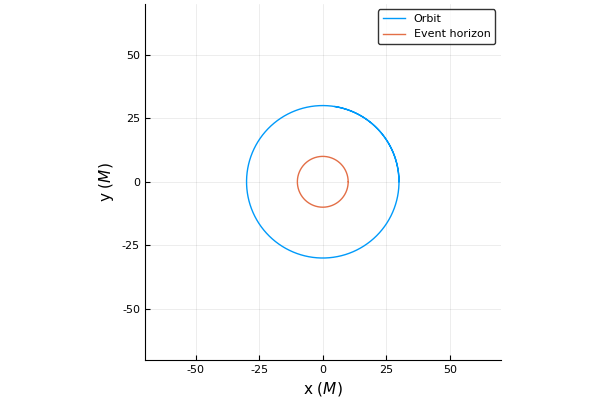
\includegraphics[width=0.45\textwidth]{images/circleorbit.png}
        \caption{A wonderfully circular orbit at 6M}
        \label{fig:circle}
    \end{figure}
    
    The nicely circular orbit in Fig.~\ref{fig:circle} pairs nicely with the relative error in the orbit with respect to the theory: of order $10^{-15}$! This is roughly the best one could get in terms of numerical errors. Fig.~\ref{fig:circleerr} shows the trend in error increase over time.

    \begin{figure}[h!]
        \centering
        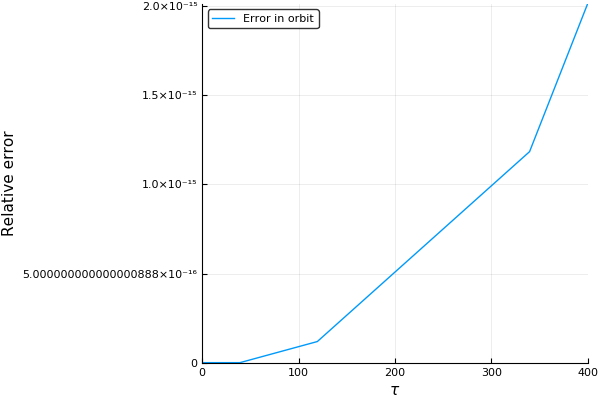
\includegraphics[width=0.45\textwidth]{images/circleorberr.png}
        \caption{Error in circular orbit}
        \label{fig:circleerr}
    \end{figure}

    The rest of the orbits that I computed can be found in the attached ``orbits.ipynb'' file.

    \section{\label{sec:discussion} Discussion}

    I wish I had started earlier or had more time to correctly implement the ADM formalism to compare the symplectic and forward integration schemes and how the manifold projection algorithm compares in accuracy with respect to the symplectic energy conservation. This was my first goal with this project, but I did not have the time to completely develop the idea. Furthermore, expanding the timelike integration part to include Doppler shift would be an essential addition to create a ray tracer, like GYOTO.\cite{GYOTO2011} However, the package is useful as it is for an example for how to implement geodesic integration in Julia. I may continue tinkering with the module in the future!

    \bibliographystyle{apsrev4-1}
    \bibliography{main}
\end{document}

